\RequirePackage{lineno} 
\documentclass[a4paper,11pt,spanish]{article}

\usepackage[spanish]{babel}
\usepackage[utf8]{inputenc}
\usepackage{url}
\usepackage{graphicx} 
\usepackage{slashbox}
\usepackage{longtable}
\usepackage{multirow}
\usepackage{colortbl}
\usepackage{color}
\usepackage{lineno}
\usepackage{tikz}
\usepackage{fancybox}


\usepackage{textcomp}
\usepackage{amsmath}
\usepackage{babel}
 

\usepackage{subfig}



% \usepackage{gantt}
% \setlength{\textheight}{24cm}
% \textwidth=16.5cm
% \topmargin=0cm
% \oddsidemargin=0cm
% \parindent=10mm
% \definecolor{shadecolor}{rgb}{1, 0, 0}
\begin{document}
%\linenumbers %activar nro de lineas
\pagestyle{empty}


\begin{center}

	\bigskip
	\bigskip
	
%	{\bf\Large Algoritmo para la detección de objetos planos aplicado a videos en un ambiente controlado.} \\
	{\bf\Large Método para detección y seguimiento de objetos con aplicaciones en Realidad Aumentada} \\
%	{\bf\Large Algoritmo para la detección de objetos planos en videos en un ambiente controlado.} \\

	\bigskip
	\bigskip

	\large Christian Nicolás Pfarher\\


  	\bigskip
  	\bigskip
	
	Punto de control N$^{\circ}$ 2: \\	
		\begin{description}
			\item Adquisición de imágenes (prototipos) para realizar las pruebas		
			\item Métodos de extracción de características en imágenes parte 1 (Análisis/estudio del método).
		\end{description}

	 
	\bigskip
	
	Director\\
	\textit{Dr. Enrique Marcelo Albornoz}\\
	\bigskip
	Codirector\\
	\textit{Dr. César Martínez}\\
	
	\bigskip
	\bigskip
	\bigskip
	\bigskip
	\bigskip
	\bigskip
	\textit{\today}\\
	

	\vfill
	\begin{figure}[tbhp]
		\centerline{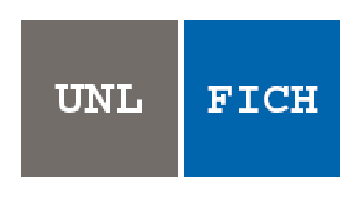
\includegraphics[scale=0.6]{img/fich_unl.eps}}
	\end{figure}
	
  	{Ingeniería Informática}\\
  	{Facultad de Ingeniería y Ciencias Hídricas}\\
    {UNIVERSIDAD NACIONAL DEL LITORAL}	
\end{center}

\bigskip
\bigskip

\newpage

\pagestyle{plain}

\section{Adquisición de imágenes (prototipos) para realizar las pruebas.}
El proceso de adquisición de imágenes es aplicado en tres diferentes instancias, según la situación:
\begin{enumerate}
  \item \textbf{Imagen patrón}: es la adquisición de la imagen que será usada como patrón para su posterior detección y seguimiento y sobre la cuál se sobre impondrá el \textbf{Objeto de Realidad Aumentada}.

  La imagen, será adquirida con la misma cámara web utilizada para la captura de la \textbf{Imagen Live}, aunque no se descarta la posibilidad del uso de otro dispositivo que permita obtener una imagen de características similares a la obtenida con la cámara web utilizada.

  La adquisición de la imagen objeto, deberá cumplir ciertas restricciones prácticas, entre las cuales se puede nombrar: el tamaño de la imagen, las condiciones de iluminación, el nivel de detalle (cantidad de detalles mínimos), entre otras.\label{imagenpatron_restricciones}

    %\begin{itemize}
    %\item \colorbox{yellow}{la imagen patrón debe ser plana}
    %\item \colorbox{yellow}{debe ocupar la totalidad de la imagen. esto se va a entender???} el tamaño de la imagen
    %\item \colorbox{yellow}{las condiciones de iluminación deben ser uniformes y sin sombras}
    %\item \colorbox{yellow}{no debe existir oclusión sobre el objeto.}
    %\item \colorbox{yellow}{la imagen debe ser tomada de forma que la normal al plano de la imagen sea ortogonal o aproximadamente ortogonal a la normal del centro de la cámara,}
    %\item \colorbox{yellow}{la imagen no tendrá blurring.}
    %\item \colorbox{yellow}{la imagen deberá poseer textura o características suficientes para ser identificada.}
    %\item \colorbox{yellow}{no debe haber brillos o reflexiones sobre la imagen -> objetos de plastico por ejemplo con luz...}
    %\item \colorbox{yellow}{si es muy chico o muy grande el objeto,.. no funciona!.... o sea si le saco a un papel de caramelo y depues lo pongo a 40 cm, no me lo detecta... a eso me refiero.. no se como se debería poner...  -- minimo de tamaño 640x480.?}
    %\item \colorbox{yellow}{textured plannar target}
    %\item \colorbox{yellow}{según esto: objetivo perdido, oclusion, inclinación, blur motion, relection}
    %\end{itemize}
 

  \item \textbf{Imagen Live o Flujo de Video}: es la obtención de un fotograma del Flujo de Video adquirido en tiempo real con la cámara web, con las mismas restricciones prácticas mencionadas anteriormente. Sobre este fotograma, se detectará la \textbf{Imagen Patrón}.

  La adquisición se realizará con una cámara web con una resolución de 640x480 píxeles de una computadora portátil Toshiba Satellite A505-S6803.
  
  \item \textbf{Objeto de Realidad Aumentada}: es la definición de una imagen (ej: foto, tapa de libro, revista, etc.) o volumen tridimensional (ej: objeto 3D dibujado con OpenGL) - dependiendo del grado de avance que se logre en el proyecto - que será sobre impuesto en el \textbf{Flujo de Video}.
  
\end{enumerate}


% \bigskip
% \textbf{Referencias de la sección:
% % \cite{cita66}, %Paul Milgram et al., 1994 
% % \cite{cita65}, %Ben Butchart, 2011
% % \cite{cita36}, %Taehee Lee et al., 2007 6dof
% % \cite{cita64}, %Ronald Azuma et al., 2001
% % \cite{5739718}.% Ahyun Lee et al., 2010  sift lkt
% }
% 
\section{Métodos de extracción de características en imágenes parte 1 (Análisis/estudio del método).}

En visión computacional, el concepto de puntos de interés, puntos claves (Keypoints) o puntos característicos (Feature Points) es usado ampliamente en diversidad de tareas tales como: el reconocimiento de objetos, la identificación de imágenes, seguimiento de objetivos, reconstrucción de escenas 3D, etc. La idea consiste en  seleccionar algunos puntos especiales de la imagen, para realizar un análisis sobre ellos. Esta aproximación es válida, en la medida en que se detecten la cantidad de puntos suficientes de tal forma que los mismos sean distinguibles y además, formen un conjunto de características estables que permitan ser precisamente localizadas en próximas observaciones.

Cuando se trata de hacer coincidir características entre diferentes imágenes (por ejemplo para el reconocimiento de las mismas), el problema del cambio de escala se hace presente. Al ser analizadas distintas imágenes, éstas,
 %Esto es, diferentes imágenes a ser analizadas, 
pueden estar tomadas a diferentes distancias respecto al objeto de interés, de tal forma que los objetos aparecen de diferentes tamaños en la imagen. Es así que, si se trata de hacer coincidir las mismas características entre dos imágenes usando un tamaño fijo de píxeles vecinos, la intensidad de los patrones no coincidirá debido al cambio de escala presente en las mismas y por lo tanto, el reconocimiento fallará.

Para solucionar este problema, el concepto de características invariantes a la escala es introducido en visión computacional. La idea central es tener un factor de escala asociada con cada punto característico detectado. 

Un detector de puntos de interés usado recientemente y basado en estas ideas es el algoritmo SURF: Speeded Up Robust Features (Detector rápido de características robustas) \cite{citeulike:9456628, citeulike:7676197, Bay:2008:SRF, bb53077, TuytelaarsM07, Bay:2008:SRF, BouGar}. Éste está basado en conceptos del algoritmo SIFT: Scale Invariant Feature Transform (Transformación de características invariante a la escala) \cite{citeulike:3484001, citeulike:9456628, citeulike:7676197, bb53077, journals/tvcg/WagnerRMDS10, TuytelaarsM07, bb48614, Nixon:2002:FEI, BouGar, 5739718, conf/ismar/SkrypnykL04}. El método SURF, no solamente tiene la característica de ser invariante a escala, sino que además, posee la ventaja de calcular eficientemente los resultados asociando una orientación con cada característica (indicado en la imagen de la figura \ref{church_difference_surf} con una línea radial dentro de cada círculo), con el objetivo de lograr invariancia respecto a la rotación.% El tamaño de los círculos de los puntos claves que se pueden observar en la figura \ref{church_difference_surf}, resulta ser proporcional a la escala de cada característica.

%%%%%%%%%%%%%%%%%%%%%%%%%%%%%%%%%%%%%%%%%%%%%%%%%%%%%%%%%%%%%%%%%%%%%%%%

\begin{figure}[tbhp]
   \centering
   %%----primera subfigura----
   \subfloat[]{
        \label{church1}         %% Etiqueta para la primera subfigura
        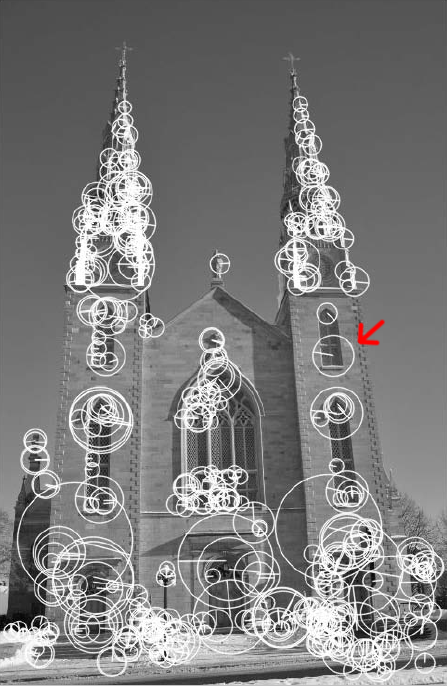
\includegraphics[scale=0.338]{img_ent2/surfinchurch1}}
   \hspace{0.1\linewidth}
   %%----segunda subfigura----
   \subfloat[]{
        \label{church2}         %% Etiqueta para la segunda subfigura
        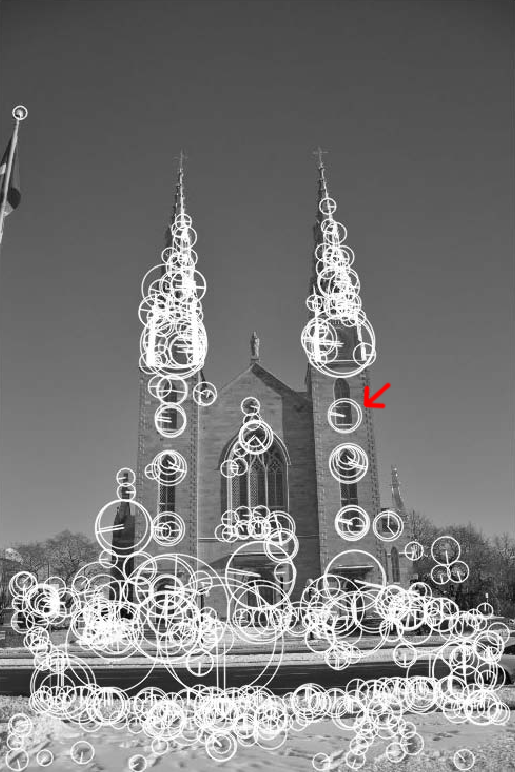
\includegraphics[scale=0.3]{img_ent2/surfinchurch2}}
    \caption{Fotografía tomada a diferentes escalas de la misma escena. (\ref{church1}) - (\ref{church2})}
   \label{church_difference_surf}                %% Etiqueta para la figura entera
\end{figure}
%

%%%%%%%%%%%%%%%%%%%%%%%%%%%%%%%%%%%%%%%%%%%%%%%%%%%%%%%%%%%%%%%%%%%%%%%%
Si se observa cuidadosamente los puntos detectados en la Fig. \ref{church_difference_surf}, se puede ver que el cambio en el tamaño de los círculos, es proporcional a los cambios de escala. Por ejemplo, si se considera la parte inferior de la ventana superior derecha de la fotografía, tanto en la Fig. \ref{church1} como en la Fig. \ref{church2}, la característica SURF ha sido detectada en la misma ubicación y los círculos correspondientes (de diferentes tamaños) contienen los mismos elementos visuales. Si bien este caso no se da para todas las características, la razón de repetición es lo suficientemente alta para permitir buenas coincidencias entre dos imágenes.
%%%%%%%%%%%%%%%%%%
\subsection{SURF - Detección de puntos claves}
La derivada de una imagen puede ser estimada mediante el uso de filtros Gaussianos, los mismos utilizan un parámetro $\sigma$ que representa la desviación estándar de la curva Gaussiana y que define la apertura del kernel. %Un filtro con un valor de $\sigma$ grande, suaviza los detalles más finos de la imagen.

Si se calcula el Laplaciano de un punto en una imagen usando filtros Gaussianos a diferentes escalas, se obtienen diferentes valores. Si miramos la evolución de las respuestas del filtro para diferentes factores de escala, se  obtiene una curva que alcanza un valor máximo en algún valor de $\sigma$ específico. Extrayéndose este valor máximo para dos imágenes del mismo objeto (tomadas a dos escalas diferentes), la relación que existe entre los $\sigma
$ máximos se corresponderán en relación con las escalas en que fueron tomadas cada una de las fotografías. Esta observación, es el núcleo del proceso de extracción de características invariantes a la escala. Es decir, que las características invariantes a escalas, pueden ser detectadas como máximos locales en el espacio imagen (localización) y en el espacio escala (obtenido de la aplicación de filtros a diferentes escalas).

SURF implementa la misma idea. Primeramente para detectar las características, se calcula la Matriz Hessiana (Hessian matrix) para cada píxel. Esta matriz mide la curvatura local de una función y tiene la forma de la matriz de la expresión (\ref{HessianMatrix}).

\begin{equation}
H(x,y)=\begin{bmatrix}\frac{\partial^{2}I}{\partial x\text{\texttwosuperior}} & \frac{\partial^{2}I}{\partial x\partial y}\\
 & \\
\frac{\partial^{2}I}{\partial x\partial y} & \frac{\partial^{2}I}{\partial y\text{\texttwosuperior}}
\end{bmatrix}\label{HessianMatrix}
\end{equation}

%El determinante de la matriz Hessiana, da la intensidad de la curva.%
La idea es por lo tanto, definir %esquinas como 
puntos de imágenes con valores de curvatura altos (esto es, alta variación en más de una dirección). Debido que la matriz está compuesta por derivadas de segundo orden, la misma puede ser calculada usando kernels Gaussianos Laplacianos de diferentes escalas $\sigma$. Así, el Hessiano pasa a ser una función de tres variables: $H(x,y,\sigma)$. Una característica invariante a la escala es identificada cuando el determinante del Hessiano alcanza un máximo local en ambos espacios (imagen y escala). %(esto es, 3x3x3 no-maximos  necesitan removerse.).%

El cálculo de todas las derivadas a diferentes escalas resulta ser costoso computacionalmente, por eso, para que el proceso resulte más eficiente se usa una aproximación a los Kernels Gaussianos conocidos como filtros caja (Boxlets filters) \cite{conf/nips/SimardBHL98} que se pueden observar en la Fig. \ref{gaussiankernels}, de forma tal que el cálculo, sólo involucre algunas operaciones de adición de enteros, reduciendo de esta forma la complejidad y permitiendo el uso de una técnica conocida como imágenes integrales \cite{viola01boosting}.

\begin{figure}[tbhp]
   \centering
   %%----primera subfigura----
   \subfloat[]{
        \label{gaussiankernelsdiscreted_y}         %% Etiqueta para la primera subfigura
        \includegraphics[scale=0.4]{img_ent2/gaussiankernelsdiscrete_y}}
	\hspace{0.1\linewidth}
   %%----segunda subfigura----
   \subfloat[]{
        \label{gaussiankernelsaprox_y}         %% Etiqueta para la segunda subfigura
        \includegraphics[scale=0.4]{img_ent2/gaussiankernelsaprox_y}}
	\hspace{0.1\linewidth}
   %%----tercera subfigura----
   \subfloat[]{
        \label{gaussiankernelsdiscreted_xy}         %% Etiqueta para la segunda subfigura
        \includegraphics[scale=0.4]{img_ent2/gaussiankernelsdiscrete_xy}}
	\hspace{0.1\linewidth}
   %%----cuarta subfigura----
   \subfloat[]{
        \label{gaussiankernelsaprox_xy}         %% Etiqueta para la segunda subfigura
        \includegraphics[scale=0.4]{img_ent2/gaussiankernelsaprox_xy}}
	\hspace{0.1\linewidth}
 \caption{Derivadas parciales Gaussianas de segundo orden discretizadas y aproximadas mediante el uso de filtros caja. Las regiones grises de la imagen son iguales a cero. - (\ref{gaussiankernelsdiscreted_y}) discretizada en la dirección ``y'', (\ref{gaussiankernelsaprox_y}) aproximada en la dirección ``y''; (\ref{gaussiankernelsdiscreted_xy}) discretizada en la dirección ``x-y'', (\ref{gaussiankernelsaprox_xy}) aproximada en la dirección ``x-y''. }             %% Etiqueta para la figura entera
  \label{gaussiankernels}
\end{figure}

El kernel de la Fig. \ref{gaussiankernels}.\ref{gaussiankernelsaprox_xy} es usado para estimar las derivadas parciales segundas, mientras que el de la Fig. \ref{gaussiankernels}.\ref{gaussiankernelsaprox_y} estima la derivada segunda en la dirección vertical. Una versión rotada de este último, estima la derivada segunda en la dirección horizontal. Los kernels más chicos (como lo de las Fig. \ref{gaussiankernels} tienen un tamaño de 9x9 píxeles, correspondiente a un $\sigma \approx 1.2$ y representa la escala más pequeña (máxima resolución espacial). % Kernels de tamaños mayores son sucesivamente aplicados.
La cantidad de filtros aplicados es especificado como un parámetro del método. Por defecto, se usan 12 diferentes tamaños de kernels (alcanzando un tamaño de 99x99). %Note que de hecho las imágenes integrales que son usadas, garantizan que la suma dentro de cada lob puede ser calculada usando solo 3 adiciones independientemente del tamaño del filtro.

Una vez que el máximo local es identificado, la posición precisa de cada punto de interés es obtenida a través de interpolación en ambos espacios (escala e imagen). El resultado es un conjunto de puntos característicos %localizados con precisión sub-pixel 
al que se le asocia una valor de escala.

\bigskip
\bigskip
\bigskip
  %%aca hay toda una serie de cosas con imágenes integrales y escalado de filtro que está más explicado en el paper pero no da para ponerlo en este informe.
\fbox{\footnotesize \parbox[c]{.9\columnwidth}{\textbf{\underline{\emph{Nota:}}} Anteriormente se ha mencionado que el algoritmo SURF ha sido desarrollado como una variante del detector de características SIFT. Este último, también detecta características como máximos locales en el espacio imagen y escala, pero usa las respuestas del filtro Laplaciano, en vez de el Determinante Hessiano. Este Laplaciano es calculado a diferentes escalas usando el filtro de Diferencia de Gaussianos. Como el cálculo de los puntos característicos esta basado en Kernels de punto flotante, el algoritmo SIFT, es considerado generalmente más preciso que SURF en términos de localización de las características en el espacio imagen y escala, pero resulta computacionalmente más costoso.}}
 %\bigskip
\subsection{Descripción de las características SURF - Vector descriptor}
Como se mencionó anteriormente, el algoritmo SURF define la localización y escala para cada una de las características detectadas. Este factor de escala, puede ser usado para definir el tamaño de una ventana alrededor de cada punto característico, de tal manera de poder definir un área vecina que incluya la misma información visual, sin importar la escala en que el objeto fue fotografiado. Así, esta información visual incluida en esa vecindad, resulta útil para caracterizar el punto y ayuda en la distinción del mismo de otros similares.

%Este capítulo, le mostrará como describir el vecindario 
Para describir el área vecina de los puntos característicos, se usan descriptores, que usualmente (en el caso de comparación entre imágenes) son vectores N-dimensionales que resultan ser invariantes a cambios de iluminación (en el caso ideal) y a pequeñas deformaciones de perspectivas. Además, resultan potencialmente usables para ser comparados mediante el uso de una métrica de distancia, como por ejemplo: la distancia euclídea.
%de los puntos caracterísiticos usando ddescriptores compactos.

 %En matching feature, \textbf{feature descriptors} son usualmente vectores N-dimensionales que describen un punto caraccterísticio,

% idealmente de una manera que es invariante a cambios en la iluminación y a deformaciones perspectivas pequeñas. 
%Además decriptores buenos pueden ser comparados mediante el uso de una métrica de distancia simple como es la distancia eculdiea por ejemplo. de hecho, esta constituye una herramienta poderosa usada en algotritmos de matching.

En el caso del algoritmo SURF, el descriptor por defecto %es de un tamaño de 
posee 64 elementos (SIFT utiliza 128 elementos) y este vector caracteriza el %patrón de intensidad %
área que rodea a un punto característico. Cuanto más similares sean los 2 puntos característicos, más cercanos serán sus vectores descriptores.



%%%%%%%%%%%%%%%%%%%%%%%%%%%%%%%%%%%%%%%%5
%% paper original:
El buen desempeño de SIFT en comparación con otros descriptores es notable. Su mezcla de información de localización %cruda
y la distribución de las características relacionadas con el gradiente, lo hacen poderoso para lograr la diferenciación de características, mientras sufre errores de localización en términos de espacio y escala. El uso de los puntos fuertes mencionados, junto con la orientación del gradiente, reduce los efectos de los cambios fotométricos. El descriptor SURF, %propuesto % 
se basa en propiedades similares, pero con su complejidad simplificada. El primer paso, consiste en fijar una orientación reproducible basada en la información de una región circular alrededor del punto de interés. Luego, se construye una región cuadrada alineada con la orientación seleccionada, y se extrae el descriptor SURF de ella.
\subsubsection{Asignación de la orientación}
\label{asignacion_orientacion_susbsection}
Con el objetivo de lograr invariancia a la rotación, se identifica una orientación que sea reproducible para los puntos de interés. Para este propósito, primeramente se calculan las respuestas de la Wavelet Harr en la dirección ``x'' y ``y'' con los kernels de la Fig. \ref{simplekernels} en una vecindad circular de radio $6\sigma$ alrededor del punto de interés (donde $\sigma$ representa la escala a la que fue detectado el punto de interés).


%%imágenes integrales y algo de la escala aclara en el paper ...
Una vez que han sido calculadas las respuestas wavelets y ponderadas por una Gaussiana centrada en el punto de interés (con un valor de $2.5\sigma$) estas son representadas mediante un vector en el espacio, con las respuestas de intensidad horizontales a lo largo de la abscisa y las verticales a lo largo de la ordenada. Para una orientación dada, las respuestas dentro de un intervalo angular ($\pi/3$) se suman, y la orientación que da el mayor vector es definido como la orientación dominante.

%La orientación dominante, es calculada como la suma de todas las respuestas dentro de una ventana deslizante con un ángulo de $\pi/3$. Las respuestas verticales y horizontales dentro de la ventana son sumadas%. Las dos respuestas sumas construyen %
%

%construyéndose así un nuevo vector. El mayor vector de entre ellos, representa la orientación del punto de interés.%
Cabe aclarar que el tamaño de la ventana deslizante es un parámetro seleccionado experimentalmente.
%%
\subsubsection{Componentes del descriptor}
Para la extracción del descriptor, el primer paso consiste en construir una región cuadrada centrada alrededor del punto de interés y orientada en la dirección de la orientación calculada en la subsección \ref{asignacion_orientacion_susbsection}. El tamaño de la ventana es $20\sigma$.

%Esta región cuadrada, es dividida en sub-regiones más pequeñas de 4x4 (muestras experimentales indican que este tamaño es con el que se obtiene mejor performance). 

%Para cada sub-región, las respuestas del kernel $dx$ y $dy$ son calculadas en un área localizada y regularmente espaciada de 5x5 (el tamaño del kernel es $2\sigma$).

La región es dividida regularmente en subregiones cuadradas más pequeñas de 4x4. Estas mantienen información espacial importante en ellas. 
Por razones de simplicidad, llamaremos $dx$ a la respuesta de la wavelet Harr en la dirección horizontal Fig. \ref{simplekernels1} y $dy$ la respuesta en la dirección vertical Fig. \ref{simplekernels2} (tamaño del filtro: $2\sigma$). ``Horizontal'' y ``Vertical'' aquí son definidas en relación a la orientación seleccionada del punto. Para incrementar la robustez frente a deformaciones geométricas y errores de localización, las repuestas $dx$ y $dy$ son primero ponderadas con un gaussiano ($3.3\sigma$) centrado en el punto de interés.

%Para cada sub-región, se calculan algunas características cada 5x5 puntos de muestreo que son mencionadas a continuación. 
\begin{figure}[tbhp]
   \centering
   %%----primera subfigura----
   \subfloat[]{
        \label{simplekernels1}         %% Etiqueta para la primera subfigura
        \includegraphics[scale=0.35]{img_ent2/simplekernels1har}}
   \hspace{0.1\linewidth}
   %%----segunda subfigura----
   \subfloat[]{
        \label{simplekernels2}         %% Etiqueta para la segunda subfigura
        \includegraphics[scale=0.35]{img_ent2/simplekernels2har}}
    \caption{Kernels aplicados en la vecindad de un punto característico.}
   \label{simplekernels}                %% Etiqueta para la figura entera
\end{figure}

Las respuestas wavelet $dx$ y $dy$ son sumadas sobre cada subregión y forman un primer conjunto de entradas para el vector de características. Con el propósito de dar información acerca de la polaridad de los cambios de intensidad, también se extrae la suma de los valores absolutos de las respuestas: $\left|dx\right|$ y $\left|dy\right|$. Así, cada subregión tiene un vector descriptor de cuatro dimensiones cuya expresión es: 
\begin{equation}
\left[\sum dx\qquad\sum dy\qquad\sum \left|dx\right|\qquad\sum \left|dy\right|\right]
\label{equation_suma} 
\end{equation} 
Esto, resulta en un vector descriptor para todas las subregiones de 4x4 de un tamaño de 64 elementos. Se debe tener en cuenta que las respuestas de las wavelets son invariantes a un sesgo en la iluminación y que la invariancia de contraste (un factor de escala) se consigue transformando el vector en uno unidad.



La Fig. \ref{respuesta_descriptor}, muestra las propiedades del descriptor para tres imágenes distintas, con diferentes patrones de intesidad, en una subregión. Una combinación de dichos patrones locales de intensidad, daría como resultado un descriptor posible de distinguir.

\begin{figure}[tbhp]
   \centering
        \includegraphics[scale=0.4]{img_ent2/egharrresponses}
    \caption{Las entradas del descriptor de una subregión, representan la naturaleza del patrón de intensidad subyacente. Izquierda: en el caso de una región homogénea, todos los valores son relativamente bajos. Centro: En presencia de frecuencias en la dirección ``x'', el valor $\sum \left|dx\right|$ es alto, mientras los demás son bajos. Derecha: Si la intensidad se incrementa gradualmente en la dirección ``x'', ambos valores: $\sum dx$ y $\sum \left|dx\right|$ son altos.}
   \label{respuesta_descriptor}                %% Etiqueta para la figura entera
\end{figure}

%%%%%%%%%%%%%%%%%%%%%%%%%%%%%%%%%%%%%%%%
%%%%%%%%%%%%%%%%%%%%%%%%%%%%%%%%%%%%%%%%%%%%%%%%%%%%%%%%%%%%%%%%%%%%%%%

% Se consideran buenos descriptores de características, a aquellos que son invariantes a pequeños cambios de iluminación, puntos de vista (perspectiva) y presencia de ruido en la imagen. Es por esto que con frecuencia, están basados en diferencias locales de intensidad. Este es el caso de los descriptores SURF, que aplican los kernels de la figura \ref{simplekernels} dentro de un área determinada %grande%
% alrededor de un punto.



%  El tamaño de la vecindad usado para extraer los vectores característicos es definido como 20 veces el factor de escala de la características (esto es, $20\sigma$). Esta región cuadrada, luego es dividida en sub-regiones más pequeñas de 4x4. Para cada sub-región, las respuestas del kernel $dx$ y $dy$ son calculadas en un área localizada y regularmente espaciada de 5x5 (el tamaño del kernel es $2\sigma$). Todas estas respuestas son sumadas mediante la expresión \ref{equation_suma} con el objetivo de extraer cuatro valores descriptivos para cada sub-región.



% Debido a que son $4x4=16$ sub-regiones, tenemos un descriptor con un total de 64 valores. Con el objetivo de dar mas importancia a los píxeles vecinos mas cercanos al punto clave, las respuestas del kernel se ponderan con un Gaussiano centrado en el punto clave (con $\sigma=3.3$).

% Las respuestas $dx$ y $dy$, son también usadas para estimar la orientación de las características. Estos valores son calculados (con un kernel de tamaño $4\sigma$) en una vecindad circular de radio $6\sigma$ en puntos regularmente espaciados por intervalos $\sigma$. Para una orientación dada, las respuestas dentro de un intervalo angular ($\pi/3$) se suman, y la orientación que da el mayor vector es definido como la orientación dominante.

De esta forma, buscar correspondencias con invariancia a escala entre imágenes es alcanzable mediante las características y descriptores que se obtiene con SURF.
%%

\bigskip
\bigskip
\bigskip

\fbox{\footnotesize \parbox[c]{.9\columnwidth}{\textbf{\underline{\emph{Aclaración respecto del algoritmo SIFT:}}} El algoritmo SIFT, también define su propio descriptor. Se basa en la magnitud del gradiente y orientación calculado en la escala del punto clave considerado. Como en el caso de los descriptores SURF, el área vecina escalada del punto clave es dividido en 4x4 subregiones. Para cada una de estas regiones, se construye un histograma de 8 clases de las orientaciones del gradiente (ponderados por su magnitud y por una ventana gaussiana global centrada en el punto clave). Luego, el vector descriptor es construido de las entradas de este histograma. Hay 4x4 regiones y 8 clases por histograma, lo que nos da un descriptor de una longitud de 128 elementos. 

En cuanto a la detección de características, la diferencia entre los descriptores SIFT y SURF es principalmente la velocidad y precisión. Mientras que los descriptores SURF están mayormente basados en diferencias de intensidades, son más rápidos de calcular; por otro lado, los descriptores SIFT son considerados generalmente más precisos en buscar la característica correcta (coincidencia más exacta), pero llevando más tiempo de cálculo.}}



%%%%%%%%%%%%%%%%%%%%%%%%%%%%%%%%%%%%%%%%%%%%%%%%%%%%%%%%%%%%%%%%%%%%%%%%%%%%%%%%%%%%%%%%%%%%%%%%%%%%%%%%%
%%%%%%%%%%%%%%%%%%%%%%%%%%%%%%%%%%%%%%%%%%%%%%%%%%%%%%%%%%%%%%%%%%%%%%%%%%%%%%%%%%%%%%%%%%%%%%%%%%%%%%%%%
%  Local Feature View Clustering for 3D Object Recognition - paper David LOWE
% Cada característica SIFT es representada por un vector con medidas locales de la imagen, de tal manera de ser invariante a la traslación, escalado y rotación y parcialmente invariante a cambios de iluminación y deformaciones locales. Una imagen típica producirá gran cantidad de características que se sobre solapen en un rango de varias escalas  que formaran una representación redundante de la imagen original. La naturaleza local y multi escala de la características la hará insensitiva al ruido, desorden y oclusiones, mientras que las propiedades de los detalles locales de la imagen representados por las características la harán altamente selectivas para realizar un match con grandes bases de datos de características previamente almacenadas.
% 
% La localización de las características SIFT son eficientemente detectadas identificando el máximo y mínimo de una función diferencia de gaussianos en el espacio escala. En cada localización, una orientación es seleccionada como el pico del histograma del gradiente de las orientaciones de la imagen local. Un vector de características es así construido mediante la medida de gradientes locales en la imagen en una región alrededor de cada punto localizando en coordenadas relativas a la localización, escala y orientación de la característica. La localización del gradiente son borroneadas para reducir la sensibilidad a pequeñas deformaciones locales de la imagen, como ser un cambio del punto de vista. Resumiendo, el enfoque de SIFT transforma las características locales de la imagen en relación con marcos de coordenadas que se espera que sean estables a través de múltiples puntos de vista de un objeto.

% El tamaño de la región de la imagen que es muestreada por cada característica es variable, pero los experimentos de este paper usan vectores de 128 elementos por cada característica para muestrear ocho orientaciones de gradientes sobre una región de 4x4. El uso de 128 elementos (un vector largo) es útil para dar un grado mayor de selectividad al hacer un maching de características con una base de datos, resultando en mejore precisión y eficiencia.
%%%%%%%%%%%%%%%%%%%%%%%%%%%%%%%%%%%%%%%%%%%%%%%%%%%%%%%%%%%%%%%%%%%%%%%%%%%%%%%%%%%%%%%%%%%%%%%%%%%%%%%%%
%%%%%%%%%%%%%%%%%%%%%%%%%%%%%%%%%%%%%%%%%%%%%%%%%%%%%%%%%%%%%%%%%%%%%%%%%%%%%%%%%%%%%%%%%%%%%%%%%%%%%%%%%

% 
% \bigskip
% \textbf{Referencias de la sección: \cite{citeulike:3484001}, %Gary Bradsky et al., 2008 
% \cite{citeulike:9456628}, %Robert Laganière, 2011
% \cite{Bay:2008:SRF},% Herbert Bay et al., 2008 surf
% \cite{TuytelaarsM07}, %Tuytelaars et al., 2008 harris, surf, klt, sitf
% \cite{bb53077}, %Krystian Mikolajczyk et al., 2005 sift, pca-sift
% \cite{journals/tvcg/WagnerRMDS10}, %Daniel Wagner et al., 2010  sift, phony sift ferns
% \cite{bb48614}, %Tsz-Wai Rachel Lo et al., 2009 sift
% \cite{cita24},% Ian Y-H Chen et al., 2008 slam OK
% \cite{Bay:2008:SRF}, %Herbert Bay et al., 2007 surf
% \cite{conf/ismar/SkrypnykL04}, %Iryna Skrypnyk et al., 2004 sift, klf
% \cite{BouGar},% Óscar Boullosa García et al., 2011  sift surf
% \cite{5739718}.% Ahyun Lee et al., 2010  sift lkt
% }
% 
% 

% %%%%%%%%%%%%%%%%%%%%%%%%%%%%%%%%%%%%%%%%%%%%%%%%%%%%%%%%%%%%%%%%%%%%%%%%%%%%%%%%%%%%%%%%%%%%%%%%%%%%%%%%%%%
\newpage
\bibliographystyle{alpha}
\bibliography{bib1,bib2,bib4}
 \end{document}
